
%(BEGIN_QUESTION)
% Copyright 2015, Tony R. Kuphaldt, released under the Creative Commons Attribution License (v 1.0)
% This means you may do almost anything with this work of mine, so long as you give me proper credit

\noindent
{\bf Lab Exercise -- introduction}

\vskip 5pt

Your team's task is to construct a relay control circuit for an AC motor, starting and stopping the motor based on the states of two process switches.  The recommended application is a {\it lift station} pump control system, where water is pumped out of a sump (bucket) according to the states of high-level and low-level switches.  Other ideas open for consideration, though.  Alternatives to this project idea are authorized by instructor permission only.

The following table of objectives show what you and your team must complete within the scheduled time for this lab exercise.  Note how some of these objectives are individual, while others are for the team as a whole:

\underbar{Objective completion table:}

% No blank lines allowed between lines of an \halign structure!
% I use comments (%) instead, so that TeX doesn't choke.

$$\vbox{\offinterlineskip
\halign{\strut
\vrule \quad\hfil # \ \hfil & 
\vrule \quad\hfil # \ \hfil & 
\vrule \quad\hfil # \ \hfil & 
\vrule \quad\hfil # \ \hfil & 
\vrule \quad\hfil # \ \hfil & 
\vrule \quad\hfil # \ \hfil & 
\vrule \quad\hfil # \ \hfil \vrule \cr
\noalign{\hrule}
%
% First row
{\bf Performance objective} & {\bf Grading} & {\bf 1} & {\bf 2} & {\bf 3} & {\bf 4} & {\bf Team} \cr
%
\noalign{\hrule}
%
% Another row
Prototype sketch ({\it before building the system!}) & mastery & -- & -- & -- & -- & \cr
%
\noalign{\hrule}
%
% Another row
Final wiring diagram and system inspection & mastery & & & & & -- -- -- -- \cr
%
\noalign{\hrule}
%
% Another row
Pictorial (layout) diagram & mastery & -- & -- & -- & -- &  \cr
%
\noalign{\hrule}
%
% Another row
Proper motor control function & mastery & -- & -- & -- & -- &  \cr
%
\noalign{\hrule}
%
% Another row
Troubleshooting & mastery & & & & & -- -- -- -- \cr
%
\noalign{\hrule}
%
% Another row
Lab question: Selection/testing & proportional &  &  &  &  & -- -- -- -- \cr
%
\noalign{\hrule}
%
% Another row
Lab question: Commissioning & proportional &  &  &  &  & -- -- -- -- \cr
%
\noalign{\hrule}
%
% Another row
Lab question: Mental math & proportional &  &  &  &  & -- -- -- -- \cr
%
\noalign{\hrule}
%
% Another row
Lab question: Diagnostics & proportional &  &  &  &  & -- -- -- -- \cr
%
\noalign{\hrule}
%
% Another row
Decommission and lab clean-up & mastery & -- & -- & -- & -- &  \cr
%
\noalign{\hrule}
} % End of \halign 
}$$ % End of \vbox

The only ``proportional'' scoring in this activity are the lab questions, which are answered by each student individually.  A listing of potential lab questions are shown at the end of this worksheet question.  The lab questions are intended to guide your labwork as much as they are intended to measure your comprehension, and as such the instructor may ask these questions of your team day by day, rather than all at once (on a single day).

\vskip 10pt

In addition to this motor control system, you must individually construct a {\it PLC trainer} for learning PLC programming.  An example is documented in the next question of this worksheet.

\underbar{PLC objective completion table:}

% No blank lines allowed between lines of an \halign structure!
% I use comments (%) instead, so that TeX doesn't choke.

$$\vbox{\offinterlineskip
\halign{\strut
\vrule \quad\hfil # \ \hfil & 
\vrule \quad\hfil # \ \hfil & 
\vrule \quad\hfil # \ \hfil & 
\vrule \quad\hfil # \ \hfil & 
\vrule \quad\hfil # \ \hfil & 
\vrule \quad\hfil # \ \hfil & 
\vrule \quad\hfil # \ \hfil \vrule \cr
\noalign{\hrule}
%
% First row
{\bf Performance objective} & {\bf Grading} & {\bf 1} & {\bf 2} & {\bf 3} & {\bf 4} & {\bf Team} \cr
%
\noalign{\hrule}
%
% Another row
All inputs (switches) function properly & mastery & & & & & -- -- -- -- \cr
%
\noalign{\hrule}
%
% Another row
All outputs (lights) function properly & mastery & & & & & -- -- -- -- \cr
%
\noalign{\hrule}
} % End of \halign 
}$$ % End of \vbox

\vskip 10pt

{\bf It is essential that your team plans ahead what to accomplish each day.  A short (10 minute) team meeting at the beginning of each lab session is a good way to do this, reviewing what's already been done, what's left to do, and what assessments you should be ready for.  There is a lot of work involved with building, documenting, and troubleshooting these working instrument systems!}

As you and your team work on this system, you will invariably encounter problems.  You should always attempt to solve these problems as a team before requesting instructor assistance.  If you still require instructor assistance, write your team's color on the lab whiteboard with a brief description of what you need help on.  The instructor will meet with each team in order they appear on the whiteboard to address these problems.




\vfil \eject

\noindent
{\bf Lab Exercise -- selecting components and planning the system}

\vskip 5pt

One of the most common problems students encounter when building any working system, whether it be a circuit on a solderless breadboard or an instrument loop spanning an entire room, is properly connecting and configuring all components.  An unfortunate tendency among most students is to simply start connecting parts together, essentially designing the system as they go.  This usually leads to improperly-connected components and non-functioning systems, sometimes with the result of destroying components due to those improper connections!

An alternative approach is to plan ahead by designing the system before constructing it.  This is easily done by sketching a diagram showing how all the components should interconnect, then analyzing that diagram and making changes before connecting anything together.  When done as a team, this step ensures everyone is aware of how the system should work, and how it should go together.  The resulting ``prototype'' diagram need not be complex in detail, but it should be detailed enough for anyone to see which component terminals (and ports) connect to terminals and ports of other devices in the system.  For example, your team's prototype sketch should be clear enough to determine all DC electrical components will have the correct polarities.  If your proposed system contains a significant amount of plumbing (pipes and tubes), your prototype sketch should show all those connections as well.

\vskip 10pt

Your first step should be selecting proper components from the instrument storage area to use in building your system.  In this particular lab, you are looking for an electric motor, pushbutton switches, process switches (e.g. liquid level-sensing switches for a lift station), and a control relay.

After locating suitable components, you should qualitatively test them prior to construction of your system.  For an electric motor, this means powering it to see that it runs.  For switches, ohmmeter (``continuity'') measurements will tell you if the switch contacts are actuating as they should.  For the control relay, you may power the coil and measure continuity with your ohmmeter to ensure the contacts are functioning properly.  If any component fails to respond properly, notify the instructor and then tag it with a label explaining what it does (or what it fails to do).

\vskip 10pt

Your team's prototype sketch is so important that the instructor will demand you provide this plan before any construction on your team's working system begins.  {\it Any team found constructing their system without a verified plan will be ordered to cease construction and not resume until a prototype plan has been drafted and approved!}  Each member on the team should have ready access to this plan (ideally possessing their own copy of the plan) throughout the construction process.  Prototype design sketching is a skill and a habit you should cultivate in school and take with you in your new career.

\vskip 10pt

{\bf Planning a functioning system should take no more than an hour if the team is working efficiently, and will save you hours of frustration (and possible component destruction!).}









\vfil \eject

\noindent
{\bf Lab Exercise -- building the system}

\vskip 5pt

The Instrumentation lab is set up to facilitate the construction of working control systems, with over a dozen junction boxes, pre-pulled signal cables, and ``racks'' set up with 2-inch vertical pipes for mounting instruments.  The only wires you should need to install to build a working system are those connecting the field instrument to the nearest junction box, and then small ``jumper'' cables connecting different pre-installed cables together within intermediate junction boxes.

After getting your prototype sketch approved by the instructor, you are cleared to begin building your system.  Locate the motor control relay inside a junction box installed on one of the racks, with the motor and process switches located nearby.  Locate the pushbutton switch (Manual start) at some other location such as the main control panel for the lab.  This ensures a long enough cable run for the switches to make the system realistic for testing and troubleshooting.  

Make absolutely sure your system is securely grounded (all metal surfaces connected to earth ground through the grounding prong on the power cord, or alternatively to a copper grounding bus on the nearest utility column.  Your installation needs to have a professional appearance with as little exposed wiring as possible!

\vskip 10pt

{\bf Common mistakes:}

\begin{itemize}
\item{} Neglecting to test individual components with a multimeter before installing them.
%\item{} Improper pipe/tube fitting installation (e.g. trying to thread tube fittings into pipe fittings and vice-versa).
\item{} Failing to tug on each and every wire where it terminates to ensure a mechanically sound connection.
\item{} Students working on portions of the system in isolation, not sharing with their teammates what they did and how.  It is important that the whole team learns all aspects of their system!
\end{itemize}

\vskip 10pt

{\bf Building a functioning system should take no more than one full lab session (3 hours) if all components are readily available and the team is working efficiently!}





\vfil \eject

\noindent
{\bf Lab Exercise -- documenting the system}

\vskip 5pt

Each student must sketch their own {\it wiring diagram} for their team's system, showing all control and power wire connections for the entire system.  A sample wiring diagram is shown on the next page.  These wiring diagrams must be {\it comprehensive} and {\it detailed}, showing every wire connection, every cable, every terminal block, etc.  The principle to keep in mind here is to make the wiring diagram so complete and unambiguous that anyone can follow it to see what connects to what, even someone unfamiliar with industrial instrumentation.  In industry, systems are often constructed by contract personnel with limited understanding of how the system is supposed to function.  The wiring diagrams they follow must be so complete that they will be able to connect everything properly without necessarily understanding how it is supposed to work.

Every wire in your system needs to be labeled with a number.  Wires electrically common to each other at all times (i.e. connected at terminal blocks, not passing through any component) must bear the same label number.  An easy way to label wires is to wrap a short piece of masking tape around each wire then writing on that masking tape with a permanent marker.  Furthermore, each number or other label appearing on a device terminal (e.g. the screw terminals on an octal-base relay socket) must be shown on your wiring diagram in parentheses, to distinguish those labels from wire numbers used to identify wires.  With each wire and each device terminal clearly labeled, one cannot go wrong in re-connecting wires that were undone.  This is important when technicians remove components for repair and replacement, as the wiring diagram is their only guide to proper re-connection of the new or repaired components.

When your entire team is finished drafting your individual wiring diagrams, call the instructor to do an inspection of the system.  Here, the instructor will have students take turns going through the entire system, with the other students checking their diagrams for errors and omissions along the way.  During this time the instructor will also inspect the quality of the installation, identifying problems such as frayed wires, improperly crimped terminals, poor cable routing, missing labels, lack of wire duct covers, etc.  The team must correct all identified errors in order to receive credit for their system.  

After successfully passing the inspection, each team member needs to place their wiring diagram in the diagram holder located in the middle of the lab behind the main control panel.  When it comes time to troubleshoot another team's system, this is where you will go to find a wiring diagram for that system!

\vskip 10pt

{\bf Common mistakes:}

\begin{itemize}
\item{} Forgetting to label all wires (see example wiring diagram).
\item{} Forgetting to label all field instruments with their own tag names (e.g. PT-83).
\item{} Forgetting to note all wire colors.
\item{} Forgetting to put your name on the wiring diagram!
\item{} Basing your diagram off of a team-mate's diagram, rather than closely inspecting the system for yourself.
\end{itemize}

\vskip 10pt

{\bf Creating and inspecting accurate wiring diagrams should take no more than one full lab session (3 hours) if the team is working efficiently!}

\filbreak

$$\includegraphics[width=15.5cm]{i03654x01.eps}$$










\vfil \eject

\noindent
{\bf Lab Exercise -- troubleshooting}

\vskip 5pt

The most challenging aspect of this lab exercise is {\it troubleshooting}, where you demonstrate your ability to logically isolate a problem in the system.  All troubleshooting is done on an individual basis (no team credit!), and must be done {\it on a system you did not help build}, so that you must rely on wiring diagrams to find your way around the system instead of from your own memory of building it.

Each student is given a limited amount of time to identify both the general location and nature of the fault, logically justifying all diagnostic steps taken.  All troubleshooting activities will take place under direct instructor supervision to ensure students are working independently and efficiently. 

Failure to correctly identify both the general location and nature of the fault within the allotted time, and/or failing to demonstrate rational diagnostic procedure to the supervising instructor will disqualify the effort, in which case the student must re-try with a different fault.  Multiple re-tries are permitted with no reduction in grade.

A standard multimeter is the only test equipment allowed during the time limit.  No diagnostic circuit breaks are allowed except by instructor permission, and then only after correctly explaining what trouble this could cause in a real system.  

The instructor will review each troubleshooting effort after completion, highlighting good and bad points for the purpose of learning.  Troubleshooting is a skill born of practice and failure, so do not be disappointed in yourself if you must make multiple attempts to pass!  One of the important life-lessons embedded in this activity is how to deal with failure, because it {\it will} eventually happen to you on the job!  There is no dishonor in failing to properly diagnose a fault after doing your level best.  The only dishonor is in taking shortcuts or in giving up.

\vskip 10pt

{\bf Common mistakes:}

\begin{itemize}
\item{} Neglecting to take measurements with your multimeter.
\item{} Neglecting to check other measurements in the system (e.g. pressure gauge readings).
\item{} Incorrectly interpreting the loop diagram (e.g. thinking you're at the wrong place in the system when taking measurements).
\item{} Incorrect multimeter usage (e.g. AC rather than DC, wrong range, wrong test lead placement).  This is especially true when a student comes to lab unprepared and must borrow someone else's meter that is different from theirs!
\end{itemize}

\vskip 10pt

{\bf Remember that the purpose of the troubleshooting exercise is to foster and assess your ability to intelligently diagnose a complex system.  Finding the fault by luck, or by trial-and-error inspection, is not a successful demonstration of skill.  The only thing that counts as competence is your demonstrated ability to logically analyze and isolate the problem, correctly explaining all your steps!}

\vskip 10pt

{\bf Troubleshooting takes a lot of lab time, usually at least two 3-hour lab sessions for everyone in a full class to successfully pass.  Be sure your team budgets for this amount of time as you plan your work, and also be sure to take advantage of your freedom to observe others as they troubleshoot, to better learn this art.}




\vfil \eject

\noindent
{\bf Lab questions}

\vskip 5pt

\begin{itemize}
\item{} {\bf Selection and Initial Testing}
\item{} Explain the meanings of the various ratings specified on the motor nameplate
\item{} Explain the meanings of the coil and contact ratings specified on the relay nameplate
\item{} Explain the different between the {\it pull-in} and {\it drop-out} voltage for a relay coil
\item{} Identify the various pins on the control relay, and corresponding terminals on the relay socket, based on the diagram shown on the relay case (or in the manufacturer datasheet for the relay)
\item{} Explain how to test the proper operation of one of the process switches on a test bench (i.e. before it is used in the motor control circuit)
\end{itemize}

\filbreak

\begin{itemize}
\item{} {\bf Commissioning and Documentation}
\item{} Demonstrate how to isolate potentially hazardous energy in your system ({\it lock-out, tag-out}) and also how to safely verify the energy has been isolated prior to commencing work on the system
\item{} Demonstrate proper use of wire strippers
\item{} Demonstrate proper use of compression terminal crimping tool
\item{} Explain importance of lockout/tagout procedure when working on power circuits
\item{} Explain what {\it arc flash} and {\it arc blast} are, and what causes these effects
\item{} Identify multiple locations (referencing a wiring diagram) where you should be able to measure full DC voltage at all times
\item{} Identify multiple locations (referencing a wiring diagram) where you should be able to measure full AC voltage at all times
\end{itemize}

\filbreak

\begin{itemize}
\item{} {\bf Mental math} (no calculator allowed!)
\item{} Convert horsepower rating of a single-phase AC electric motor into a current rating (at a specified line voltage)
\item{} Convert current rating of a single-phase AC electric motor into a horsepower rating (at a specified line voltage)
\end{itemize}

\filbreak

\begin{itemize}
\item{} {\bf Diagnostics}
\item{} ``Virtual Troubleshooting'' -- referencing their system's diagram(s), students propose diagnostic tests (e.g. ask the instructor what a meter would measure when connected between specified points; ask the instructor how the system responds if test points are jumpered) while the instructor replies according to how the system would behave if it were faulted.  Students try to determine the nature and location of the fault based on the results of their own diagnostic tests.
\item{} Explain how to distinguish an ``open'' cable fault from a ``shorted'' cable fault using only a voltmeter (no current or resistance measurement, but assuming you are able to break the circuit to perform the test)
\item{} Determine whether or not a given diagnostic test will provide useful information, given a set of symptoms exhibited by a failed system
\item{} Identify at least two plausible faults given the results of a diagnostic test and a set of symptoms exhibited by a failed system
\end{itemize}


\vfil \eject

\noindent
{\bf Lab Exercise -- decommissioning and clean-up}

\vskip 5pt

The final step of this lab exercise is to decommission your team's entire system and re-stock certain components back to their proper storage locations, the purpose of which being to prepare the lab for the next lab exercise.  Remove your system documentation (e.g. loop diagram) from the common holding area, either discarding it or keeping it for your own records.  Also, remove instrument tag labels (e.g. FT-101) from instruments and from cables.

\vskip 10pt

\indent
{\bf Leave the following components in place, mounted on the racks:}

\begin{itemize}
\item{} Large electric motors
\item{} Large variable-frequency drive (VFD) units
\item{} Cables inside conduit interconnecting junction boxes together
\item{} Pipe and tube fittings (do not unscrew pipe threads)
\item{} Supply air pressure regulators
\end{itemize}

\vskip 10pt

\indent
{\bf Return the following components to their proper storage locations:}

\begin{itemize}
\item{} Process switches
\item{} Manual (e.g. pushbutton) switches
\item{} ``Jumper'' cables used to connect terminal blocks within a single junction box
\item{} Plastic tubing and tube fittings (disconnect compression-style tube fittings)
\item{} Power cables and extension cords
\item{} Adjustment (loading station) air pressure regulators
\end{itemize}



\underbar{file i03654}
%(END_QUESTION)





%(BEGIN_ANSWER)


%(END_ANSWER)





%(BEGIN_NOTES)

\noindent
{\bf Loop diagrams / inspections:}

I strongly recommend checking off students' loop diagrams while you inspect their loop (checking for secure wiring, proper tubing, good conduit installation, etc.) with them.  Have all team members take you on a ``tour'' of their completed loop, with each team member explaining a different portion of the loop you select while using their own loop diagram as a guide.  While a student is explaining their section of the loop, you can check the other students' loop diagrams for accuracy.  This not only saves time by consolidating the tasks of loop inspection and loop diagram verification, but it also ensures students can actually relate their loop diagrams to the loop they have built and articulate that understanding to you.

\vskip 10pt

\goodbreak

\noindent
{\bf Troubleshooting fault ideas:}

\begin{itemize}
\goodbreak
\item{} Strip wire at terminal, then insert insulated wire end under terminal and tighten (open wire fault)
\item{} Cut signal cable somewhere in mid-conduit (open wire fault)
\item{} Push a thumbtack through the cable somewhere in mid-conduit (shorted wire fault)
\item{} Wire instrument cable conductors backward (construction fault)
\item{} Configure transmitter for excessive damping (slow response fault)
\item{} Configure indicator/controller for excessive damping (slow response fault)
\item{} Miscalibrate transmitter and/or indicator/controller (inaccuracy fault)
\item{} Plug tube connections using portion of foam earplug stuffed into tube fitting (slow response fault)
\item{} Reverse action of controller/positioner/transmitter (wrong response fault)
\item{} Mis-configure linear/sq.root characterization of transmitter and/or indicator/controller (nonlinearity fault)
\item{} Connect 2.2 k resistor in parallel with 4-20 mA transmitter to simulate partial short in wiring (inaccuracy fault)
\item{} Exchange 250 ohm resistor for a different resistor that looks the same but has the wrong value (inaccuracy fault) 
\item{} Unplug cable(s) inside transmitter or controller (failed instrument fault)
\item{} Give students wrong loop diagram (documentation fault)
\item{} Start students out on wrong controller (operator error)
\item{} Close valve and leave safety tag hanging on it (operator/technician error)
\end{itemize}

%INDEX% Lab exercise, motor control circuit (relay-based)

%(END_NOTES)


